\documentclass[a4paper, 11pt]{article}
\usepackage[UTF8, scheme = plain]{ctex}
\usepackage{xcolor}     %高亮使用的颜色
\definecolor{commentcolor}{RGB}{85,139,78}
\definecolor{stringcolor}{RGB}{206,145,108}
\definecolor{keywordcolor}{RGB}{34,34,250}
\definecolor{backcolor}{RGB}{220,220,220}
\usepackage{accsupp}	
\newcommand{\emptyaccsupp}[1]{\BeginAccSupp{ActualText={}}#1\EndAccSupp{}}
\usepackage{amsmath}
\usepackage{graphicx}
\usepackage{geometry}
\usepackage{listings}
\usepackage[colorlinks,linkcolor=red]{hyperref}
\geometry{scale=0.8}

\title{	
\normalfont \normalsize
\textsc{School of Data and Computer Science, Sun Yat-sen University} \\ [25pt] %textsc small capital letters
\rule{\textwidth}{0.5pt} \\[0.4cm] % Thin top horizontal rule
\huge  E2 15-Puzzle Problem (IDA*)\\ % The assignment title
\rule{\textwidth}{2pt} \\[0.5cm] % Thick bottom horizontal rule
\author{18308045 Zhengyang Gu}
\date{\normalsize\today}
}

\begin{document}
\maketitle
\tableofcontents
\newpage

\section{IDA* Algorithm}
\subsection{Description}
Iterative deepening A* (IDA*) was first described by Richard Korf in 1985, which is a graph traversal and path search algorithm that can find the shortest path between a designated start node and any member of a set of goal nodes in a weighted graph.

It is a variant of \textbf{iterative deepening depth-first search} that borrows the idea to use a heuristic function to evaluate the remaining cost to get to the goal from the \textbf{A* search algorithm}.

Since it is a depth-first search algorithm, its memory usage is lower than in A*, but unlike ordinary iterative deepening search, it concentrates on exploring the most promising nodes and thus does not go to the same depth everywhere in the search tree.

\textbf{Iterative-deepening-A* works as follows:} at each iteration, perform a depth-first search, cutting off a branch when its total cost $f(n)=g(n)+h(n)$ exceeds a given threshold. This threshold starts at the estimate of the cost at the initial state, and increases for each iteration of the algorithm. At each iteration, the threshold used for the next iteration is the minimum cost of all values that exceeded the current threshold.
\subsection{Pseudocode}
\begin{figure}[ht]
	\centering
	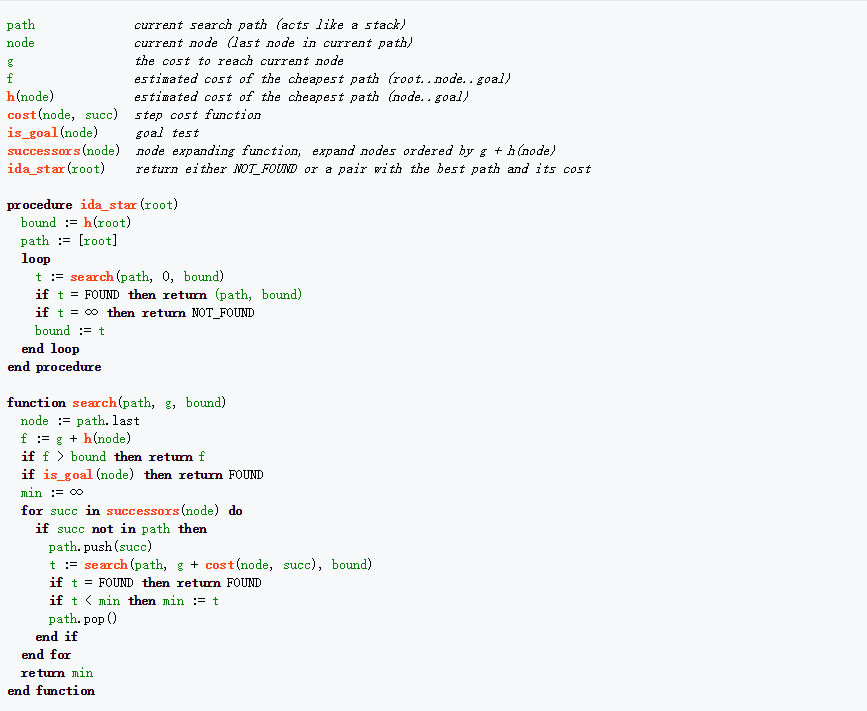
\includegraphics[width=17.3cm]{Pic/code}
\end{figure}
\section{Tasks}



\begin{itemize}
	\item Please solve 15-Puzzle problem by using IDA* (Python or C++). You can use one of the two commonly used heuristic functions: h1 = the number of misplaced tiles. h2 = the sum of the distances of the tiles from their goal positions.
	\item Here are 4 test cases for you to verify your algorithm correctness. You can also play this game (\texttt{15puzzle.exe}) for more information.
	      \begin{figure}[ht]
		      \centering
		      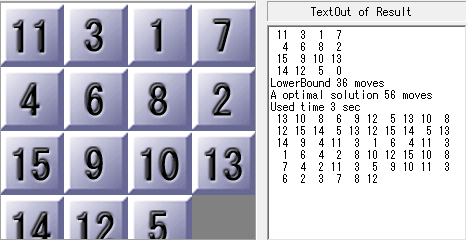
\includegraphics[width=8cm]{Pic/case1}
		      \quad
		      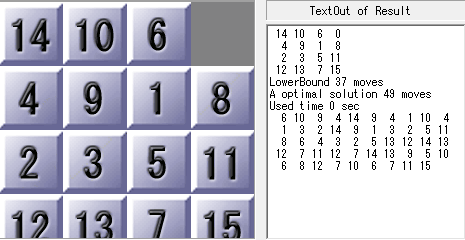
\includegraphics[width=8cm]{Pic/case2}
		      \\
		      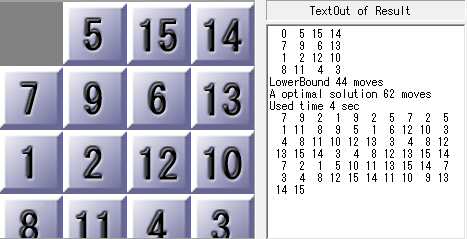
\includegraphics[width=8cm]{Pic/case3}
		      \quad
		      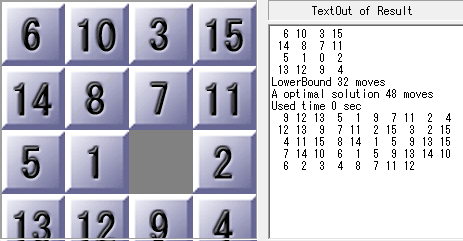
\includegraphics[width=8cm]{Pic/case4}

	      \end{figure}
	\item Please send \texttt{E02\_YourNumber.pdf} to \texttt{ai\_2020@foxmail.com}, you can certainly use \texttt{E02\_15puzzle.tex} as the \LaTeX template.
\end{itemize}


\section{Codes}
%%\lstset{language=C++}
\lstset{						%高亮代码设置
	language=python, 					%Python语法高亮
	linewidth=0.95\linewidth,      		%列表list宽度
	%basicstyle=\ttfamily,				%tt无法显示空格
	commentstyle=\color{commentcolor},	%注释颜色
	keywordstyle=\color{keywordcolor},	%关键词颜色
	stringstyle=\color{stringcolor},	%字符串颜色
	%showspaces=true,					%显示空格
	numbers=left,						%行数显示在左侧
	numberstyle=\tiny\emptyaccsupp,		%行数数字格式
	numbersep=5pt,						%数字间隔
	frame=single,						%加框
	framerule=0pt,						%不划线
	escapeinside=@@,					%逃逸标志
	emptylines=1,						%
	xleftmargin=3em,					%list左边距
	backgroundcolor=\color{backcolor},	%列表背景色
	tabsize=4,							%制表符长度为4个字符
	gobble=4,							%忽略每行代码前4个字符
}
\begin{lstlisting}
	import time
	path = list()
	# @通过值查目标位置@
	goal_reverse = ((3, 3), (0, 0), (0, 1), (0, 2),
					(0, 3), (1, 0), (1, 1), (1, 2),
					(1, 3), (2, 0), (2, 1), (2, 2),
					(2, 3), (3, 0), (3, 1), (3, 2))
	row = 4
	col = 4
	range_row = range(row)
	range_col = range(col)
	puzzle = list()
	# @曼哈顿距离,只调用一次,后续动态修改f值@
	def h():
		ans = 0
		for i in range_row:
			for j in range_col:
				if puzzle[i][j] is 0:
					continue
				goal_pos = goal_reverse[puzzle[i][j]]
				ans += abs(i - goal_pos[0]) + abs(j - goal_pos[1])
		return ans
	cost = 1
	# @通过位置查目标值@
	goal = ((1, 2, 3, 4),
			(5, 6, 7, 8),
			(9, 10, 11, 12),
			(13, 14, 15, 0))
	def is_goal():
		for i in range_row:
			for j in range_col:
				if puzzle[i][j] is 0:
					continue
				if puzzle[i][j] is not goal[i][j]:
					return False
		return True
	# @记录0所在的位置,方便更新@
	zero_pos
	directions = ((-1, 0), (1, 0), (0, -1), (0, 1))
	def successors():
		global zero_pos
		ans = list()
		for direction in directions:
			succ = (zero_pos,
					(zero_pos[0] + direction[0],
					zero_pos[1] + direction[1]))
			if 0 <= succ[1][0]\
					and succ[1][0] < row\
					and 0 <= succ[1][1]\
					and succ[1][1] < col:
				ans.append(succ)
		return ans
	# @当前图的hash值,可以放入set中用于路经检测@
	# @list类型的puzzle无法放入set中@
	cur_hash = 0
	# @初始化cur\_hash,后续只对变化元素修改cur\_hash@
	def hash():
		global cur_hash
		base = 1
		for i in range_row:
			for j in range_col:
				cur_hash += base * puzzle[i][j]
				base *= 16
	inf = float("inf")
	vis = set()
	def ida_star():
		global zero_pos
		stt = h()
		bound = stt
		vis.add(hash())
		for i in range_row:
			for j in range_col:
				if puzzle[i][j] is 0:
					zero_pos = (i, j)
					break
			else:
				continue
			break
		while 1:
			t = search(path, stt, bound)
			if t is True:
				return (path, bound)
			if t == inf:
				return False
			bound = t 
	def search(path, f, bound):
		global zero_pos
		global cur_hash
		if f > bound:
			return f
		if is_goal():
			return True
		min = inf
		for succ in successors():
			succ_value = puzzle[succ[1][0]][succ[1][1]]
			last_hash = cur_hash
			cur_hash += succ_value
			* (16 ** (succ[0][0] * col + succ[0][1])
			- 16 ** (succ[1][0] * col + succ[1][1]))
			puzzle[succ[0][0]][succ[0][1]] = succ_value
			puzzle[succ[1][0]][succ[1][1]] = 0
			zero_pos = succ[1]
			if cur_hash not in vis:
				path.append(succ)
				vis.add(cur_hash)
				goal_pos = goal_reverse[succ_value]
				t = search(path,
							f + abs(succ[0][0] - goal_pos[0]) +
							abs(succ[0][1] - goal_pos[1])
							- (abs(succ[1][0] - goal_pos[0]) +
								abs(succ[1][1] - goal_pos[1])) + cost,
							bound)
				if t is True:
					return True
				if t < min:
					min = t
				vis.remove(cur_hash)
				path.pop()
			zero_pos = succ[0]
			puzzle[succ[1][0]][succ[1][1]] = succ_value
			puzzle[succ[0][0]][succ[0][1]] = 0
			cur_hash = last_hash
		return min
	def read_15puzzle(file_name):
		with open(file_name) as f:
			for i in range_row:
				line = f.readline()
				if not line:
					break
				puzzle.append([int(i) for i in line.split()])
	read_15puzzle("test4.txt")
	for i in puzzle:
		for j in i:
			print(j, end = '\t')
		print()
	start = time.perf_counter()
	ans = ida_star()
	end = time.perf_counter()
	print("Time used:", end - start)
	print(ans)
\end{lstlisting}
\section{Results}
\begin{figure}[ht]
	\centering
	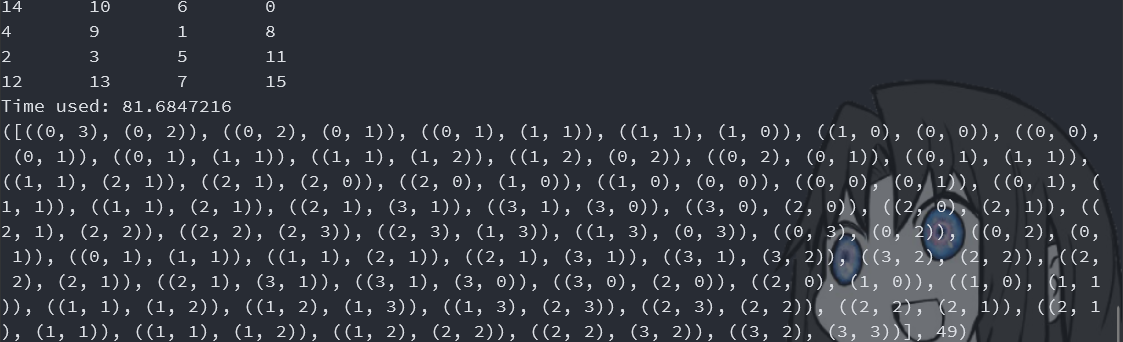
\includegraphics[width=12cm]{result2.png}
	\caption{result2}
	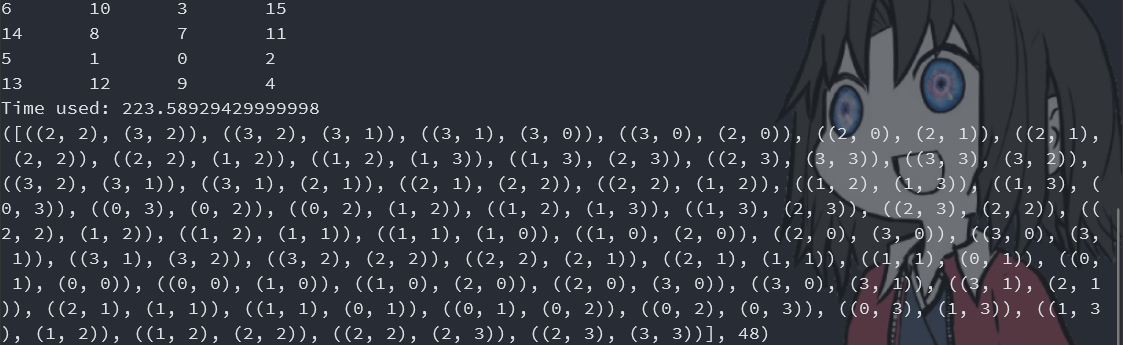
\includegraphics[width=12cm]{result4.png}
	\caption{result4}
\end{figure}

%\clearpage
%\bibliography{E:/Papers/LiuLab}
%\bibliographystyle{apalike}
\end{document}